\documentclass[a4paper,DIV=12,10pt]{scrartcl}

\usepackage{graphicx}
\usepackage{color}
\usepackage{booktabs}
\usepackage{tabularx}
\usepackage{comment}
\usepackage{tikz}
\usepackage{standalone}
\usepackage{minted}  % source code highlighting
\usepackage{textcomp}

%%------------------------------------------------------------------------------
%% Includes for math features
\usepackage[intlimits]{amsmath}
\usepackage{amssymb}
\usepackage{commath} % dif operators
\usepackage{mathtools}
\usepackage{stmaryrd}

%%------------------------------------------------------------------------------
%% Math macros
%%------------------------------------------------------------------------------
\newcommand{\vek}[1]{\boldsymbol{#1}}  %% make argument bold (any font)
\newcommand{\mat}[1]{\mathsf{#1}}      %% use sans-serif font for math
\newcommand{\jump}[1]{\llbracket #1 \rrbracket} %% jump of argument
\newcommand{\avg}[2]{\{ #1 \}_{#2}}             %% average formula
\newcommand{\defeq}{\vcentcolon=} %% :=  for equal-def
\newcommand{\col}[0]{\vcentcolon}

\DeclareMathOperator{\tr}{tr}
%% include notes style file

\graphicspath{{./pics/}}

%%------------------------------------------------------------------------------
\newcommand{\x}[0]{\vek{x}}
\newcommand{\X}[0]{\vek{X}}
\newcommand{\xxi}[0]{\vek{\xi}}
\newcommand{\U}[0]{\vek{u}}
\newcommand{\V}[0]{\vek{v}}
\newcommand{\N}[0]{\vek{n}}

\newcommand{\IS}[0]{\texttt{inSilico}}

\renewcommand{\thefootnote}{\fnsymbol{footnote}}

\newcommand{\TILDE}[0]{$\thicksim$}

\usepackage[colorlinks=true,linkcolor=blue]{hyperref} 
%%------------------------------------------------------------------------------

\begin{document}

\author{Thomas R\"uberg}
\date{\today}
\title{\texttt{inSilico} Tutorial}
\maketitle

\tableofcontents{}

\subsection*{Notation}
Throughout the text bold-typed letters indicate a point or a vector
in~$\mathbb{R}^d$, e.g. \mbox{$\x = (x_1, \dotsc, x_d)$}. Sans serif letters
denote matrices (or vectors as column-matrices), e.g. \mbox{$\mat{A} =
\{A_{KL}\}$} with some index ranges for~$K$ and~$L$. Moreover, the
following abbreviations are introduced in the text and frequently
used:
\begin{itemize}
\item FEM --- Finite Element Method
\item BVP --- Boundary Value Problem
\item IBVP --- Initial Boundary Value Problem
\item ODE  --- Ordinary Differential Equation\,.
\end{itemize}

\section{Theoretical background}
\label{sec:fem}

The Finite Element Method (FEM) is one of many numerical techniques
for the approximate solution of boundary value problems (BVP). Such
BVPs are commonly mathematical models of physical problems and a wide
range of such problems has been successfully analysed by means of
FEM. Even though the method's main application background is in the
field of structural analysis and solid mechanics, its applicability
goes far beyond these fields.

\subsection{Abstract boundary value problem and weak form}
\label{sec:bvp}


In order to go through the main characteristics of the method, some
abstract notation will be used in the following. Specific examples
follow in the tutorial sections~\ref{sec:diffusion}
to~\ref{sec:fluid}. 
%
\begin{figure}[hbtp]
  \centering
  \def\tikzscale{1.5}
  \documentclass[tikz]{standalone}

\usepackage{tikz}

\def\tikzscale{.7}
\begin{document}


\begin{tikzpicture}[scale=\tikzscale]

  %%\draw[black,fill=blue!20!white]
  %%(0,0) rectangle (5,4);
  
  \begin{scope}[shift={(1,2)}]
    \draw[blue!50!black,thick,fill=red!20!white]
    (0,0) 
    .. controls +( 0.0, 0.5) and +(-0.5, 0.1) .. (1.0, 1.0)
    .. controls +( 0.5,-0.1) and +(-0.5, 0.0) .. (2.0, 0.8)
    .. controls +( 0.5, 0.0) and +( 0.1, 0.5) .. (3.0, 0.0)
    .. controls +(-0.1,-0.5) and +( 0.5, 0.0) .. (2.0,-1.1)
    .. controls +(-0.5, 0.0) and +( 0.4, 0.0) .. (1.0,-1.0)
    .. controls +(-0.4, 0.0) and +( 0.0,-0.5) .. (0.0, 0.0);
  \end{scope}

  %\node[text=blue] at (0.4,0.4) {$\Omega^2$};
  \node[text=red]  at (3.0,2.0) {$\Omega$};
  \node[text=blue!50!black] at (2.0,3.2) {$\Gamma$};
  
  \draw[blue!50!black,thick,->] (3.8,1.5) -- node[near end,above]
  {$\mathbf{n}$} +(0.5,-0.25);

\end{tikzpicture}

\end{document}

%%% Local Variables: 
%%% mode: latex
%%% TeX-master: t
%%% End: 

  \caption{Model domain~$\Omega$ with boundary~$\Gamma$}
  \label{fig:domain}
\end{figure}
%
Let~$\Omega$ denote a domain embedded in~$\mathbb{R}^d$ and
let~$\Gamma = \partial \Omega$ be its boundary, see
figure~\ref{fig:domain}. Moreover, the boundary~$\Gamma$ is
partitioned in two regions~$\Gamma^D$ and~$\Gamma^N$ such that~$\Gamma
= \Gamma^D \cup \Gamma^N$. We are interested in the values of a
function~$u$ in~$\Omega$, where this function fulfils the following
BVP
\begin{equation}
  \label{eq:bvp}
  \begin{aligned}
    L u &= f  \qquad &\x &\in \Omega \\
    u &= g^D  &\x &\in \Gamma^D \\
    T_{\N} u &= g^N &\x &\in \Gamma^N\,.
  \end{aligned}
\end{equation}
Here, $L$ and~$T_{\N}$ are (linear) differential operators. $f$ is a body
force or source term function, $g^D$ is function that prescribes~$u$
on the boundary part~$\Gamma^D$ (\emph{Dirichlet} condition) and~$g^N$
is function that prescribes~$T_{\N} u$ on the boundary part~$\Gamma^N$
(\emph{Neumann} condition). In case of inconvenience with this
notation, refer to table~\ref{tab:physical} for some common physical
examples. 

\begin{table}[htbp]
  \centering
  {\footnotesize
    \begin{tabular}{rccccc}
      \toprule
      &$u$/$g^D$ &$g^N$ &$f$ &$Lu$ &$T_{\N}u$ \\
      \midrule
      heat &temperature $\theta$ &heat flux &heat source &$-\kappa
      \nabla^2 \theta$ &$\kappa \N \cdot \nabla \theta$ \\
      linear elasticity &displacement $\U$ &traction &body force 
      &$-\mu \nabla\!\cdot\!\nabla \U - (\lambda+\mu) \nabla \nabla\!\cdot\!\U$
      &$[\mu \nabla \U + (\lambda +\mu) \nabla \U^\top]\!\cdot\!\N$ \\
      \bottomrule
    \end{tabular}
  }
  \caption{Physical examples for the notation of the abstract boundary
    value problem~\eqref{eq:bvp}.}
  \label{tab:physical}
\end{table}

The paramount ingredient in the derivation of a finite element
formulation is the \emph{weak form} which will now be
introduced. Therefore take another function~$v$ (called \emph{test
  function}) which is zero on the boundary
part~$\Gamma^D$.\footnote{There are regularity requirements on~$v$
  (and on~$u$ in the first place) which are not discussed here.}  Now
the residual of the partial differential equation in~\eqref{eq:bvp},
i.e. \mbox{$L u - f = 0$}, is multiplied (weighted) by~$v$ and the
whole term is integrated over the domain~$\Omega$. Then
\emph{integration by parts}\footnote{Recall the divergence theorem
  $\int_\Omega \nabla \cdot \U \dif \x = \int_\Gamma \U \cdot \N \dif
  s$.} gives the desired expression. This approach (\emph{weighted
  residual method}) reads
\begin{equation}
  \label{eq:wr}
  \int_\Omega (L u -f) v \dif \x = 
  a(u,v) - \int_\Omega f v \dif \x -\int_{\Gamma^N} (T_{\N} u) v \dif s = 
  a(u,v) - \int_\Omega f v \dif \x - \int_{\Gamma^N} g^N v \dif s = 0\,.
\end{equation}
Note that $v=0$ on~$\Gamma^D$ and thus the integral over that
boundary part vanishes, and on~$\Gamma^N$ the value of~$T_{\N} u$ is
prescribed by~$g^N$. It remains to explain the ominous object~$a(u,v)$
appearing in equation~\eqref{eq:wr}. This is a bilinear form which
means that it is linear in both arguments (e.g., $a(\alpha u_1 + \beta
u_2, v) = \alpha a(u_1,v) + \beta a(u_2,v)$) and its result is a real
number. Obviously these facts are not very helpful and we consider the
expressions for~$a(u,v)$ for the cases given in
table~\ref{tab:physical}
\begin{align*}
  \text{heat:} 
  &&a(\theta,v) = \int_\Omega \kappa \nabla \theta \cdot \nabla v  \dif \x \\
  \text{elasticity:} 
  &&a(\U,\V) =\int_\Omega \vek{\sigma}(\U) \col \vek{\varepsilon}(\U)
  \dif \x
\end{align*}
with the stress tensor~$\vek{\sigma}$ and the linear strain~$\vek{\varepsilon}$.
The weak form~\eqref{eq:wr} is the foundation of the \emph{variational
  principle}:
\begin{equation}  \label{eq:vp}
  \begin{multlined}[c][.8\displaywidth]
    \text{Find $u$ with $u=g^D$ on $\Gamma^D$ such that} \\
    a(u,v) = \int_\Omega f v \dif \x + \int_{\Gamma^N} g^N v \dif s \\
    \text{for all $v$ with $v = 0$ on $\Gamma^D$}
  \end{multlined}
\end{equation}
which is the basis of any standard finite element formulation.

%%------------------------------------------------------------------------------
\subsection{Spatial discretization}
\label{sec:spatial}

The overall task is to find an approximation~$u_h$\footnote{The letter
  $h$ refers to a characteristic size of the elements introduced
  below. The notion $\lim_{h\to 0} \|u_h - u\| = 0$ is what is
  commonly understood as convergence of the method.}  for the
solution~$u$ of the BVP~\eqref{eq:bvp}. The most common approach in
FEM is the trial
\begin{equation}
  \label{eq:trial}
  u_h(\x) = \sum u^K \varphi_u^K(\x) \,,
\end{equation}
that is a linear combination of unknown coefficients~$u^K$ and
predefined functions~$\varphi_u^K$. The functions~$\varphi_u^K$ form the essence
of any FEM and will be introduced in the following. 

First, the domain~$\Omega$ of our mathematical model~\eqref{eq:bvp} is
decomposed in small convex polytopes. Note that this process (commonly
referred to as \emph{triangulation}) is in general an
approximation. Let~$\tau_e$ denote the~$e$-th of in total~$N_e$
polytopes. Then we have the expression
\begin{equation}
  \label{eq:domain}
  \Omega \approx \Omega_h = \bigcup_{e=1}^{N_e} \tau_e
\end{equation}
which states that~$\Omega$ is approximated by~$\Omega_h$ which itself
is the union of all polytopes~$\tau_e$. The triangulation
of~$\Omega_h$ is called the grid or \emph{mesh} and the individual
polytopes are referred to as \emph{elements}.  For sake of clarity,
the polytopes are of the type
\begin{description}
\item[$d=1$:] line elements,
\item[$d=2$:] triangle or quadrilateral elements,
\item[$d=3$:] tetrahedron or hexahedron elements.
\end{description}
Recall that~$d$ is the spatial dimension of the problem.

The next step is to introduce \emph{shape functions}. These usually
serve three purposes
\begin{itemize}
\item representation of the geometry of~$\Omega_h$
  \begin{equation}
    \label{eq:geometry}
    \x_h = \sum \x^M \varphi^M_{\x} \,,
  \end{equation}
\item the trial~\eqref{eq:trial}, 
\item and as test functions $v = \varphi^L_v$.
\end{itemize}
In many, but not all, circumstances it is customary to set $\varphi^K_u =
\varphi^K_v$, i.e. to use the same functions for the
trial~\eqref{eq:trial} and as test functions. Moreover, especially in
structural analysis, it is common to use for the geometry
representation the same functions as for the trial, i.e. $\varphi_{\x}^K =
\varphi_u^K$. This latter simplification is referred to as
\emph{isoparametric}. Unless specified otherwise, we will use the
notation
\begin{equation}
  \label{eq:isoparam}
  \varphi^K \defeq \varphi^K_u = \varphi^K_v = \varphi^K_{\x}\,.
\end{equation}

But what are now these~$\varphi$? In most cases, one introduces a
so-called \emph{reference element}~$\hat{\tau}$, which can be mapped
to any of the elements~$\tau_e$ of the triangulation of~$\Omega_h$
\begin{equation}
  \label{eq:map}
  T_e: \quad \xi \ni \hat{\tau} \to \x_h(\xi) \in \tau_e\,.
\end{equation}
The most standard approach is to use polynomials
on~$\hat{\tau}$. Examples are the linear functions on line, triangle
or tetrahedron elements which assume the value 1 at one vertex and 0
at the other vertices. For quadrilateral elements, the corresponding
shape functions with the same feature would be bilinear.  The shape
function on an element~$\tau_e$ result from the inverse coordinate map
of shape functions~$\hat{\varphi}$ defined on the reference element
\begin{equation}
  \label{eq:shapefun}
  \varphi^K(\x)|_{\tau_e} = \hat{\varphi}^K( \xi(\x) ) 
  = (\hat{\varphi}^K \circ T_e^{-1})(\x)
\end{equation}
and, in general, lose their polynomial character. The precise
definitions of shape functions is given in any standard text book on
FEM and will not be considered here any further.

For most physical fields, it is standard to request a certain
regularity of the solution~$u$ that carries over to its
approximate~$u_h$. The continuity of~$u_h$ across the boundaries of
adjacent elements is a very frequently imposed condition. For the
example of the linear shape functions, this condition is imposed by
requiring a unique value~$u^K$ at every vertex~$K$ of the triangulation.

In the variational principle~\eqref{eq:vp} it was required that $u =
g^D$ and $v =0$ on~$\Gamma^D$. This way of imposing boundary
conditions is called \emph{essential}. The standard way for imposing
these conditions is to set $u^K = g^D(\x^K)$ for all vertices $\x^K \in
\Gamma^D$ and to discard any test function $v = \varphi^K$ for the same
set of vertices. Note that this approach is very restricted since the
following requirements have to be fulfilled
\begin{itemize}
\item $\varphi^K(\x^K) = 1$ and $\varphi^L(\x^K) = 0$ for all other $L \neq
  K$, and
\item $\x^K \in \Gamma^D$ (note that $\x^K$ is a vertex of the
  approximate geometry and not necessarily lies on the true boundary
  $\Gamma^D$).
\end{itemize}
Whereas the latter condition is often and successfully discarded the
former can be a severe restriction. We define two index sets
\begin{equation}
  \label{eq:indexSets}
    \mathbb{I} = \{ K\col \quad \x^K \in \Omega_h \text{ and }
    \x^K \notin \Gamma_h^D \} \,,\qquad
    \mathbb{J} = \{ K\col \quad \x^K \in \Gamma_h^D \}\,,
\end{equation}
introduce the coefficients
\begin{equation}
  \label{eq:syscoeff}
  A_{KL} = a( \varphi^L, \varphi^K ) \,, \qquad
  b_K    = \int_{\Gamma_h^N} g^N \varphi^K \dif s + \int_{\Omega_h} f
  \varphi^K \dif s\,,
\end{equation}
and the matrices
\begin{equation}
  \label{eq:matrices}
  \mat{A} = \{ A_{KL} \}_{K,L \in \mathbb{I}}\,, \qquad
  \mat{x} = \{ u^K \}_{K \in \mathbb{I}} \,, \qquad
  \mat{b} = \{b_K - \sum_{L \in \mathbb{J}}
  A_{KL} u^L \}_{K \in \mathbb{I}}\,.
\end{equation}
Note the appearance of the prescribed coefficients~$u^L$, $L \in
\mathbb{J}$, in the definition of~$\mat{b}$. Finally, we have a system 
\begin{equation}
  \label{eq:system}
  \mat{A} \mat{x} = \mat{b}
\end{equation}
whose solution yields the unknown coefficients~$u^K$, $K \in
\mathbb{I}$, and the trial~\eqref{eq:trial} gives the approximate
solution~$u_h$ at any point $\x \in \Omega_h$.

%%------------------------------------------------------------------------------
\subsection{Temporal discretization}
\label{sec:temporal}

The BVP~\eqref{eq:bvp} does not depend on time and therefore the
solution of system~\eqref{eq:system} gives the time-constant state of
the physical problem to analyse. Now we consider temporal variations
for the time interval~$[0,T]$ in the following
form\footnote{Other temporal variations are possible,
  e.g. higher-order derivatives, varying domain $\Omega(t)$ or viscous
  material laws.}
\begin{equation}
  \label{eq:ibvp}
  \begin{aligned}
    \rho \partial_t u + L u &= f \qquad 
    &\x &\in \Omega\,, &t &\in [0,T]\\
    u &= g_D    &\x &\in \Gamma^D\,, &t &\in [0,T]\\
    T_{\N}u &= g_N &\x &\in \Gamma^N\,, &t &\in [0,T]\\
    u &= u_0    &\x &\in \Omega\,, &t &=0 \,.
  \end{aligned}
\end{equation}
With respect to the BVP~\eqref{eq:bvp}, the differences are: appearance
of the first time derivative~$\partial_t u$ multiplied by the material
density~$\rho$, the initial condition (last equation above) and the
time dependency of all involved quantities. Problem~\eqref{eq:ibvp} is
usually called an \emph{initial} boundary value problem (IBVP).  Since
its solution~$u(\x,t)$ is now a function of space and time, so is its
approximate~$u_h(\x,t)$. There are various approaches to tackle the
time variation. Here we follow the approach of first discretizing in
space and then applying a finite difference method to the resulting
system of ordinary differential equations (ODE). 
The starting point of this approach is rewrite the trial~\eqref{eq:trial}
\begin{equation}
  \label{eq:ttrial}
  u_h(\x,t) = \sum u^K(t) \varphi_u^K(\x) \,,
\end{equation}
with time-dependent coefficients. Following now the steps of
section~\ref{sec:spatial} leads to the system
\begin{equation}
  \label{eq:ode}
  \mat{M} \dot{\mat{x}} + \mat{A} \mat{x} = \mat{b}\,,
\end{equation}
where the \emph{mass} matrix has been introduced which is defined as
\begin{equation}
  \label{eq:mass}
  \mat{M} = \{M_{KL}\}_{K,L \in \mathbb{I}}\,,\quad
  M_{KL} = \int_{\Omega_h} \rho \varphi^K \varphi^L \dif \x\,.
\end{equation}
System~\eqref{eq:ode} is now represented by the simple (ODE)
\begin{equation}
  \label{eq:simpleOde}
  \dot{y} = f(y,t)\,.
\end{equation}
A huge variety of methods exists for the numerical solution of this
ODE and we will restrict ourselves to the family of linear multi-step
methods. Let the considered time interval~$[0,T]$ be subdivided
into~$N$ pieces of size~$\Delta t$.\footnote{The size of the time
  steps $\Delta t$ does not need to be constant but we assume this
  simpler form here.}  The~$n$-th multiple of~$\Delta t$ is the time
point $t^n = n \Delta t$ and the evaluation of the (approximate)
quantities at this point is denoted by using~$n$ as a superscript,
$f^n = f(y^n, t^n)$ and $y^n \approx y(t^n)$. Assume that all
quantities at~$t^m$, $m \leq n$ are given and the values at~$t^{n+1}$
are now of interest.  A linear multi-step method gives the equation
\begin{equation}
  \label{eq:multistep}
  \sum_{s=0}^A a_s y^{n+1-s} = \Delta t\sum_{s=0}^B b_s f^{n+1-s}\,.
\end{equation}
The number of terms~$A$ and~$B$ for the left and right side,
respectively, and the coefficients~$a_s$ and~$b_s$ are determined by
the choice of method. Expression~\eqref{eq:multistep} can be carried
over to system~\eqref{eq:ode} and gives a sequence of linear systems
of equations to solve, one for every time point~$t^n$.

%%------------------------------------------------------------------------------
\subsection{\texttt{inSilico} --- A generic Finite Element library}
\label{sec:insili}

\IS{} is a software \emph{library}, that means it is designed to serve
as a code development platform. It is \emph{not} a FEM solver package,
like \texttt{ABAQUS}. If you want to use \IS, you need to program an
application code yourself!

\IS{} is programmed in \texttt{C++} and makes heavily use of
\emph{templates}. In order to get an idea of templates, consider the
example given in figure~\ref{fig:template}. It shows two possible
template-based ways to implement the computation of the maximum of two
numbers. The important feature is that neither the class nor the
function knows of which specific type~\texttt{T} is. Therefore, they can
be employed in the software for any data type that allows the
\emph{less than} comparison based on the \texttt{operator$<$}.

\begin{figure}[htbp]
  \centering
  \begin{minted}[frame=bottomline]{c++}
template<typename T> 
struct Max {
  static T apply(const T& a, const T& b)
  { 
    return (a > b? a : b );
  }
};
//usage (Note: explicit instantiation)
const double maximum = Max<double>::apply( 3.1, -1.2 );
  \end{minted} 
  \begin{minted}[]{c++}
template<typename T>
T max(const T& a, const T& b)
{
  return (a > b? a : b);
}
//usage (Note: argument dependent look-up)
const int    maxInt = max( 3,   -1   );
const double maxDob = max( 3.1, -1.2 );
  \end{minted}

  \caption{A template class (top) and a template function (bottom) for
  the computation of the maximum of two numbers; usage examples are given.}
  \label{fig:template}
\end{figure}

This seemingly simple example hints at the power hidden behind the
concept of template-based programming: properly designed code
units have to be defined only once for a certain task.  In the
example in the bottom of figure~\ref{fig:template} the function is
used for two different number types without the need of writing a
max-function for \texttt{int} and \texttt{double} separately.  Two
important remarks have to be made at this point:
\begin{itemize}
\item The second version looks neater, since the user only has to call
  that function and the type of~\texttt{T} is implicitly determined by
  the argument types of function. This concept is called
  \emph{argument dependent look-up}. Note that it fails if the types
  cannot be uniquely determined from the argument types.
\item Compilers are usually not very good in reporting a compilation
  error in a template-based code. Try compiling the example code for a
  complex number type (no $<$-comparison available) and enjoy the
  lengthy output.
\end{itemize}

Another potential of templates is the use of parameters instead of
types, which, for instance, is commonly used for fixed-size arrays. An
illustrative example is the template-based meta-programming as shown
in figure~\ref{fig:meta}. Here, the factorial of a number~$n$ is
computed. Note that the factorial has two possible definitions which
obviously give the same result,
\begin{equation*}
  n! = \prod_{i=1}^n i = 1 \times 2 \times \dots \times n 
  \qquad \text{or} \qquad
  n! = n (n-1)!\,, \quad 0! = 1\,.
\end{equation*}
Note that the standard way (top of figure~\ref{fig:meta}) exactly
reflects the first definition of the factorial. The second, recursive
definition is represented by the meta-program (bottom of the figure).
The advantage of this way is that the compiler will compute the
factorial and effectively write its result into the compiled
program. Thereby no run-time is consumed for this computation. 
It has to be emphasised that
\begin{itemize}
\item The value of the parameter of a template has to be known at
  compile time. In the example, it is not possible to compute~$n!$
  if~$n$ is a value that is asked from the user of the program.
\end{itemize}

\begin{figure}[htbp]
  \centering
        \begin{minted}[frame=bottomline]{c++}
unsigned factorial( const unsigned n ) 
{
  unsigned result = 1;
  for ( unsigned i = 2; i <= n; i++) result *= i;
  return result;
}

const unsigned facN = factorial( N ); //usage
  \end{minted}
  \begin{minted}{c++}
template<unsigned N> struct Factorial // recursive template
{
  static const unsigned value = N * Factorial<N-1>::value;
};

template<> struct Factorial<0> // recursion stop
{
  static const unsigned value = 1;
};

//usage:
const unsigned facN = Factorial<N>::value; //N is known at compile-time
  \end{minted}

  \caption{Traditional way (top) and meta-program (bottom) to compute the factorial.}
  \label{fig:meta}
\end{figure}

The library \IS{} uses these concepts whenever possible. Consider for
example the node class as displayed in figure~\ref{fig:node}. The
class itself depends on the spatial dimension \texttt{DIM} which
determines the size of the coordinate the node holds. The exact type
used for that coordinate, defined elsewhere in the library, shall not
matter. Since the spatial dimension of the physical problem is
something that is known at the beginning and does not change in the
computation, it is an ideal candidate for a template
parameter. Moreover, the class holds two template functions for the
change and the access of the coordinate. Basically, the components of
the coordinate are copied from or to an iterator which goes over some
storage specified by the caller. This could refer to an array or
something more complicated, but does not affect the design of the node
class due to the template functions.

\begin{figure}[htbp]
  \centering
  \begin{minted}{c++}
template<unsigned DIM>
class Node
{
public:
    //! Template parameter: spatial dimension
    static const unsigned dim = DIM;

    //! Coordinate type definition
    typedef typename base::Vector<dim>::Type VecDim;

    //! Constructor
    Node()
        : id_( base::invalidInt ),
          x_(  base::invalidVector<dim>() )
    { }

    //--------------------------------------------------------------------------
    //! Set the global ID
    void setID( const std::size_t id ) { id_ = id; }
    //! Set coordinates from iterator
    template<typename INPITER>
    void setX( INPITER iter )
    {
        for ( unsigned d = 0; d < dim; d ++ ) x_[d] = *iter++;
    }

    //--------------------------------------------------------------------------
    //! Return global ID of node
    std::size_t getID() const { return id_; }
    //! Pass coordinates to an iterator
    template<typename OUTITER>
    void getX( OUTITER iter ) const
    {
        for ( unsigned d = 0; d < dim; d ++ ) *iter++ = x_[d];
    }
    
private:
    std::size_t id_; //!< Global Node ID
    VecDim      x_;  //!< Coordinate of this node
};
  \end{minted}
  \caption{Reduced version of the node class in \IS.}
  \label{fig:node}
\end{figure}


The design rationale of \IS{} is to separate data storage from
algorithms. In line with this idea is the concept to abstract finite
elements from the physical specifications. The main module of \IS{} is
the \texttt{base} module which contains all the data structures and
algorithms necessary for a finite element analysis without
specification of any physical model. On the other hand, the modules of
\texttt{heat}, \texttt{solid}, and \texttt{fluid} contain the integral
kernels as the they appear in the corresponding physical models of
heat conduction (or diffusion), elasticity and viscous fluid flow.
Figure~\ref{fig:structure} shows the top level structure of \IS{} and
the sub-modules given in \texttt{base}.

\begin{figure}[htbp]
  \centering
  \begin{minipage}[t]{0.6\textwidth}
    \vspace{0pt}
    \documentclass{standalone}

\usepackage{tikz}

\begin{document}
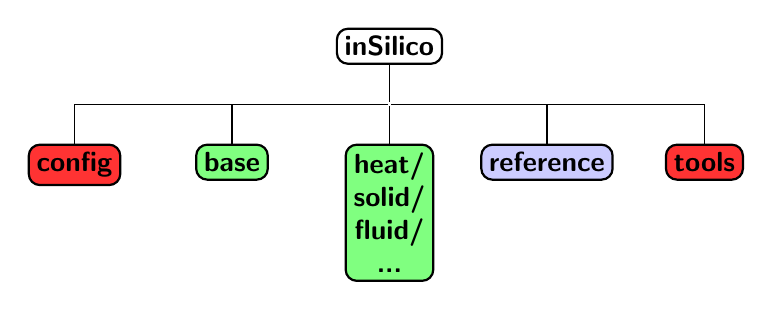
\begin{tikzpicture}
  
  \node[anchor=center,inner sep=-1mm] (X) at (0,0) {};

  % node styles
  \tikzstyle{Box}=[
  anchor=north,
  thick,
  font=\sffamily\bfseries,
  align=center,
  inner sep=1mm,
  shape=rectangle,rounded corners,draw]

  \tikzstyle{Label}=[font=\sffamily\bfseries\tiny]

  \draw (X) node[Box,anchor=south] (I)  at +( 0.0,  0.5) {inSilico};

  \draw (X) node[Box,fill=  red!80] (C)  at +(-4.0, -0.5) {config};
  \draw (X) node[Box,fill=green!50] (B)  at +(-2.0, -0.5) {base};
  \draw (X) node[Box,fill=green!50] (M)  at +( 0.0, -0.5) {heat/\\solid/\\fluid/\\...};
  \draw (X) node[Box,fill= blue!20] (R)  at +( 2.0, -0.5) {reference};
  \draw (X) node[Box,fill=  red!80] (T)  at +( 4.0, -0.5) {tools};

  \draw (I.south) -- (X) -- +(-2,0) -- (B.north);
  \draw (X) ++(-2,0) -- +(-2,0) -- (C.north);
  \draw (X) -- (M.north);
  \draw (X) -- +(2,0) -- (R.north);
  \draw (X) ++(2,0) -- +(2,0) -- (T.north);

\end{tikzpicture}
\end{document}


%%% Local Variables: 
%%% mode: latex
%%% TeX-master: t
%%% End: 
\\[1cm]
    \centering
    \documentclass{standalone}

\usepackage{tikz}

\begin{document}
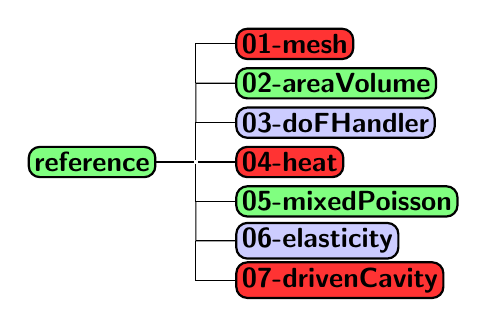
\begin{tikzpicture}
  
  \node[anchor=center,inner sep=-1mm] (X) at (0,0) {};

  % node styles
  \tikzstyle{Box}=[
  anchor=west,
  thick,
  font=\sffamily\bfseries,
  align=center,
  inner sep=0.7mm,
  shape=rectangle,rounded corners,draw]

  \tikzstyle{Label}=[font=\sffamily\bfseries\tiny]

  \draw (X) node[Box,anchor=east,fill=green!50] (I)  at +(-0.5,  0.0) {reference};

  \draw (X) node[Box,fill=  red!80] (A4)  at +(0.5, 1.5) {01-mesh};
  \draw (X) node[Box,fill=green!50] (A5)  at +(0.5, 1.0) {02-areaVolume};
  \draw (X) node[Box,fill= blue!20] (A6)  at +(0.5, 0.5) {03-doFHandler};

  \draw (X) node[Box,fill=  red!80] (A7)  at +(0.5, 0.0) {04-heat};

  \draw (X) node[Box,fill=green!50] (A8)  at +(0.5,-0.5) {05-mixedPoisson};
  \draw (X) node[Box,fill= blue!20] (A9)  at +(0.5,-1.0) {06-elasticity};
  \draw (X) node[Box,fill=  red!80] (A0)  at +(0.5,-1.5) {07-drivenCavity};

  \draw (I.east) -- (X);
  \draw (X) -- (A7.west);
  \draw (X) -- ++(0,-0.5) -- (A8.west);
  \draw (X) ++(0,-0.5) -- +(0,-0.5) -- (A9.west);
  \draw (X) ++(0,-1.0) -- +(0,-0.5) -- (A0.west);

  \draw (X) -- ++(0,0.5) -- (A6.west);
  \draw (X) ++(0,0.5) -- +(0,0.5) -- (A5.west);
  \draw (X) ++(0,1.0) -- +(0,0.5) -- (A4.west);

\end{tikzpicture}
\end{document}


%%% Local Variables: 
%%% mode: latex
%%% TeX-master: t
%%% End: 

  \end{minipage}%
  \begin{minipage}[t]{0.4\textwidth}
    \vspace{0pt}
    \documentclass{standalone}

\usepackage{tikz}

\begin{document}
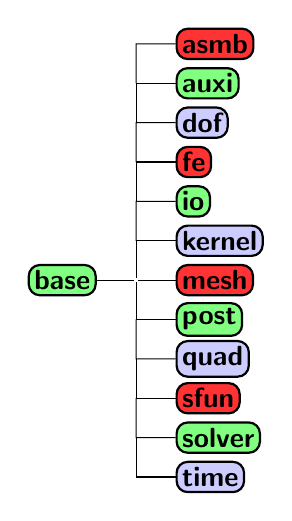
\begin{tikzpicture}
  
  \node[anchor=center,inner sep=-1mm] (X) at (0,0) {};

  % node styles
  \tikzstyle{Box}=[
  anchor=west,
  thick,
  font=\sffamily\bfseries,
  align=center,
  inner sep=0.7mm,
  shape=rectangle,rounded corners,draw]

  \tikzstyle{Label}=[font=\sffamily\bfseries\tiny]

  \draw (X) node[Box,anchor=east,fill=green!50] (I)  at +(-0.5,  0.0) {base};

  \draw (X) node[Box,fill=  red!80] (A1)  at +(0.5, 3.0) {asmb};
  \draw (X) node[Box,fill=green!50] (A2)  at +(0.5, 2.5) {auxi};
  \draw (X) node[Box,fill= blue!20] (A3)  at +(0.5, 2.0) {dof};
  \draw (X) node[Box,fill=  red!80] (A4)  at +(0.5, 1.5) {fe};
  \draw (X) node[Box,fill=green!50] (A5)  at +(0.5, 1.0) {io};
  \draw (X) node[Box,fill= blue!20] (A6)  at +(0.5, 0.5) {kernel};
  \draw (X) node[Box,fill=  red!80] (A7)  at +(0.5, 0.0) {mesh};
  \draw (X) node[Box,fill=green!50] (A8)  at +(0.5,-0.5) {post};
  \draw (X) node[Box,fill= blue!20] (A9)  at +(0.5,-1.0) {quad};
  \draw (X) node[Box,fill=  red!80] (A0)  at +(0.5,-1.5) {sfun};
  \draw (X) node[Box,fill=green!50] (AX)  at +(0.5,-2.0) {solver};
  \draw (X) node[Box,fill= blue!20] (AY)  at +(0.5,-2.5) {time};

  \draw (I.east) -- (X);
  \draw (X) -- (A7.west);
  \draw (X) -- ++(0,-0.5) -- (A8.west);
  \draw (X) ++(0,-0.5) -- +(0,-0.5) -- (A9.west);
  \draw (X) ++(0,-1.0) -- +(0,-0.5) -- (A0.west);
  \draw (X) ++(0,-1.5) -- +(0,-0.5) -- (AX.west);
  \draw (X) ++(0,-2.0) -- +(0,-0.5) -- (AY.west);

  \draw (X) -- ++(0,0.5) -- (A6.west);
  \draw (X) ++(0,0.5) -- +(0,0.5) -- (A5.west);
  \draw (X) ++(0,1.0) -- +(0,0.5) -- (A4.west);
  \draw (X) ++(0,1.5) -- +(0,0.5) -- (A3.west);
  \draw (X) ++(0,2.0) -- +(0,0.5) -- (A2.west);
  \draw (X) ++(0,2.5) -- +(0,0.5) -- (A1.west);

\end{tikzpicture}
\end{document}


%%% Local Variables: 
%%% mode: latex
%%% TeX-master: t
%%% End: 
\\[1cm]
    \fbox{
      \documentclass{standalone}

\usepackage{tikz}

\begin{document}
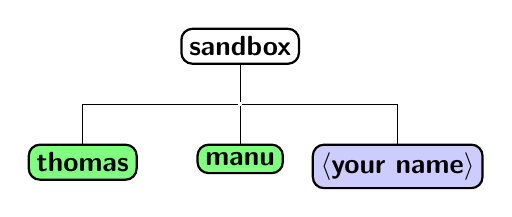
\begin{tikzpicture}
  
  \node[anchor=center,inner sep=-1mm] (X) at (0,0) {};

  % node styles
  \tikzstyle{Box}=[
  anchor=north,
  thick,
  font=\sffamily\bfseries,
  align=center,
  inner sep=1mm,
  shape=rectangle,rounded corners,draw]

  \tikzstyle{Label}=[font=\sffamily\bfseries\tiny]

  \draw (X) node[Box,anchor=south] (I)  at +( 0.0,  0.5) {sandbox};

  \draw (X) node[Box,fill=green!50] (B)  at +(-2.0, -0.5) {thomas};
  \draw (X) node[Box,fill=green!50] (M)  at +( 0.0, -0.5) {manu};
  \draw (X) node[Box,fill= blue!20] (R)  at +( 2.0, -0.5) {$\langle$your name$\rangle$};

  \draw (I.south) -- (X) -- +(-2,0) -- (B.north);
  \draw (X) -- (M.north);
  \draw (X) -- +(2,0) -- (R.north);


\end{tikzpicture}
\end{document}

%%% Local Variables: 
%%% mode: latex
%%% TeX-master: t
%%% End: 

    }
  \end{minipage}

  \caption{Directory structure of \IS: top level (top left),
    \texttt{base} module (top right), reference applications (bottom
    left) and the \texttt{sandbox}.}
  \label{fig:structure}
\end{figure}

Next to the discussed modules, there are
\begin{description}
\item[\texttt{config}:] Configuration of the software with machine
  dependent setups
\item[\texttt{tools}:] A variety of tools used in the process of the
  finite element analysis: mesh-file conversion, post-processing
  tools, etc.
\item[\texttt{reference}:] Reference applications which address
  specific parts of the library and are (partially) tested.
\end{description}
In addition, there is the \texttt{sandbox} in which random
applications can be placed and maintained. Note that the entire
library and its applications are stored within the version management
system \texttt{Subversion} on a file server. A few of the implemented
finite element features of \IS{} are given in
table~\ref{tab:features}.
\begin{table}[bthp]
  \centering
  \begin{tabular}{lp{0.75\textwidth}}
    \toprule 
    element shapes 
    &line (LINE), triangle (TRI), quadrilateral (QUAD), tetrahedron (TET),
    hexahedron (HEX)\\
    shape functions 
    &Lagrangian (linear and quadratic), B-Splines (any order)\\
    quadrature 
    &Gau\ss{}-Legendre (1- to 10-point rules), tensor-products
    for QUAD and HEX, Gau\ss{}-type quadrature for TRI and TET\\
    time integration
    &BDF and Adamas-Moulton up to fourth order \\
    solver
    &Cholesky, LU, Conjugate gradient (all via \texttt{Eigen3})\\
    \bottomrule
  \end{tabular}
  \caption{Some FEM features of \IS{}.}
  \label{tab:features}
\end{table}

At last, an abstract worflow of a finite element analysis with \IS{}
shall be outlined. A preliminary is that the steps in
figure~\ref{fig:getinstall} have already been successfully carried
out.
\begin{itemize}
\item Get a mesh file with a triangulation of the domain. The native
  format of \IS{} is \texttt{smf}, but there are two alternative ways:
  \begin{itemize}
  \item convert any other format to \texttt{smf} (a converter for
    \texttt{Gmsh} mesh files is provided in the \texttt{tools} module)
  \item write your own input method which fills the data of the
    mesh class (see \texttt{base/io/smf} for a guideline)
  \end{itemize}
\item Run an application with that mesh file. If there is no adequate application,
  do the following
  \begin{itemize}
  \item copy an existing application that you find in the
    \texttt{reference} module or somewhere in the \texttt{sandbox}
    that comes closest to your wishes
  \item modify and compile
  \end{itemize}
\item Analyse the data. The standard way is to write a \texttt{VTK}
  file which can be visualised with, e.g., \texttt{ParaView}. But
  there are many other application-specific ways to analyse the data
  a program generates.
\end{itemize}

\begin{figure}[bthp]
  \centering
  \line(1,0){450}
  \begin{enumerate}
  \item Get an account on \texttt{hermes}, read-only access to
    \IS{} and read-and-write access to the \texttt{sandbox}
  \item Create a local system folder where you want to place the
    library (e.g. \texttt{makedir \TILDE/inSilico})
  \item Enter that folder (\texttt{cd \TILDE/inSilico}) and get the \IS{}
    library  (\texttt{svn checkout
      '\url{https://web.hermes.cps.unizar.es/repos/m2be/InSilico}'})
  \item Do the same with the sandbox
    (\url{https://web.hermes.cps.unizar.es/repos/m2be/Sandbox}) 
  \item Install the external libraries
    \begin{itemize}
    \item \texttt{Eigen3} (\url{http://bitbucket.org/eigen/eigen/get/3.1.3.tar.gz})
    \item \texttt{boost}
      (\url{https://sourceforge.net/projects/boost/files/boost/1.53.0/boost_1_53_0.tar.gz})
    \end{itemize}
  \item Adapt the settings in \texttt{config.default} file (in \TILDE/inSilico/config).
  \item Try to compile the reference applications and conversion tools
  \end{enumerate}
  \line(1,0){450}
  \caption{How to get and install \IS{}.}
  \label{fig:getinstall}
\end{figure}

%%------------------------------------------------------------------------------
\newpage
\section{Tutorial problems}

\subsection{Diffusion}
\label{sec:diffusion}

Consider the diffusion IBVP
\begin{equation}
  \label{eq:diffusion}
  \begin{aligned}
    \rho \partial_t c - \kappa \nabla^2 c &= f  \qquad
    &\x &\in \Omega\,, &t &\in [0,T]\\
    c &= \bar{c}
    &\x &\in \Gamma^D\,, &t &\in [0,T]\\
    q \defeq -\kappa \nabla c \cdot \N &= \bar{q}
    &\x &\in \Gamma^N\,, &t &\in [0,T]\\
    c &= c_0
    &\x &\in \Omega\,, &t &= 0\,.
  \end{aligned}
\end{equation}
This problem describes the concentration~$c$ of some substance at
point~$\x$ and time~$t$ due to given initial and boundary conditions.
The material parameters are the density~$\rho$ and the diffusion
coefficient~$\kappa$. On the boundary part~$\Gamma^D$, the
concentration is set to~$\bar{c}$ and on the remaining boundary
part~$\Gamma^N$ the boundary flux~$q = - \kappa \nabla c \cdot \N$ is
prescribed as~$\bar{q}$. Initially, a concentration distribution~$c_0$
is assumed.

The domain~$\Omega$ is the microfluidic device depicted in
figure~\ref{fig:microfluidic} and the boundary parts~$\Gamma^D$
and~$\Gamma^N$ are described by via coordinate functions as specified
in the program. Figure~\ref{fig:inp1} shows the input parameters read
by the program.

\begin{figure}[htbp]
  \centering
  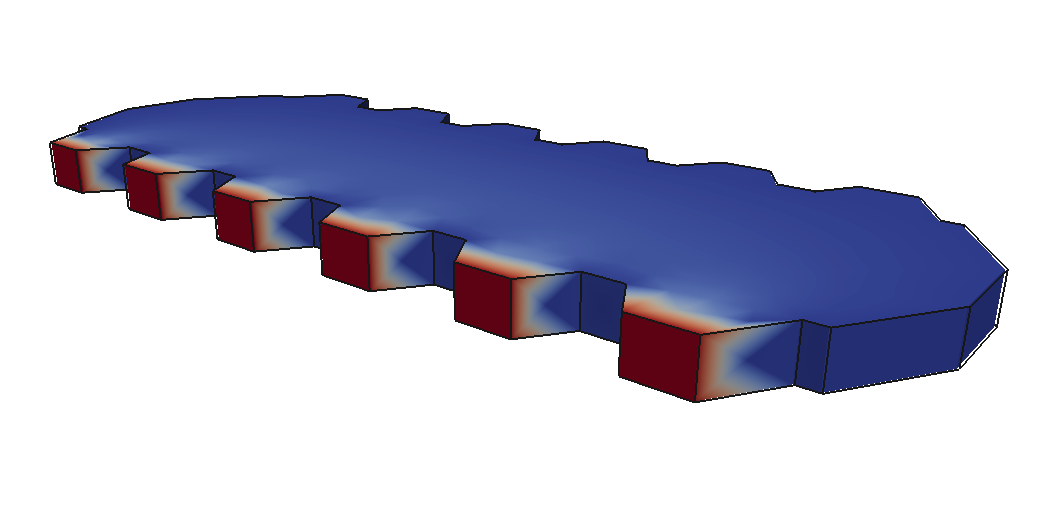
\includegraphics[width=.5\textwidth]{microfluidic}
  \caption{Microfluidic device}
  \label{fig:microfluidic}
\end{figure}

\begin{figure}[htbp]
  \centering
  \begin{minted}[frame=lines]{text}
# mesh file
meshFile   microfluidic.smf

# material conductivity
kappa      1.0

# material density
rho        1.0

# time integration stuff
numSteps   50
stepSize   0.01
  \end{minted}

  \caption{Input data of the program.}
  \label{fig:inp1}
\end{figure}

In this tutorial, two types of analyses are considered: steady and
unsteady. In the first case, the time derivative
in~\eqref{eq:diffusion} is discarded and the parameters corresponding
to a time-dependent analysis from the input file in
figure~\ref{fig:inp1} are ignored. In either case the class
\texttt{BoundarValueProblem} as given in figure~\ref{fig:bvp} is used
by the code. This class defines which boundary regions are~$\Gamma^D$
and which are $\Gamma^N$ in function of the provided
coordinate. Moreover, the boundary data~$\bar{c}$ and~$\bar{q}$, the
force function~$f$ and the initial state~$c_0$ are provided by this
class. If changes are made to \texttt{BoundarValueProblem}, the
program has to be recompiled before they apply.

\begin{figure}[htbp]
  \centering
  {\small
  \begin{minted}{cpp}
template<unsigned DIM>
struct BoundaryValueProblem
{
    static const unsigned dim = DIM;    // spatial dimension
    STATIC_ASSERT_MSG( dim == 3, "Implementation requires dim=3" );
    // convenience typedefs
    typedef typename base::Vector<DIM>::Type VecDim;
    typedef typename base::Vector<1>::Type   VecDoF;

    // boundary points with x_1 > 0.7 are on the Neumann boundary
    // or top and bottom points;
    static bool isNeumann( const VecDim & x ) 
    {
        const bool minX = ( std::abs( x[0] + 0.5 ) < coordTol );
        const bool maxX =  x[0] > 0.7;
        const bool maxZ = ( std::abs( x[2] - 0.    ) < coordTol ) or
                          ( std::abs( x[2] + 0.145 ) < coordTol );
        return maxX or ( maxZ and not minX );
    }
    static bool isDirichlet( const VecDim& x ) { return not(isNeumann( x ));}

    // boundary points with x_1 = -0.5 have a non-zero value
    static bool hasAppliedValue( const VecDim& x )
    {
        return std::abs( x[0] + 0.5 ) < coordTol;
    }

    // Dirichlet boundary condition
    template<typename DOF>
    static void dirichleBC( const VecDim& x, DOF* doFPtr )
    {
        const double appliedValue = 1.0; 
        if ( isDirichlet( x ) ) {
            const double value = (hasAppliedValue(x) ? appliedValue : 0. );
            if ( doFPtr -> isActive(0) ) doFPtr -> constrainValue( 0, value );
        }
    }

    // Body force function
    static VecDoF forceFun( const VecDim& x )
    {
        return base::constantVector<1>( 0. );
    }

    // Flux boundary condition
    static VecDoF neumannBC( const VecDim& x, const VecDim& normal )
    {
        return base::constantVector<1>( 0. );
    }

    // Initial condition
    template<typename DOF>
    static void initialState( const VecDim& x, DOF* doFPtr ) 
    {
        doFPtr -> setValue( 0, 0.0 );
    }
};
\end{minted}
}
  \caption{Class for description of the boundary value problem's given data.}
  \label{fig:bvp}
\end{figure}



%%------------------------------------------------------------------------------
\newpage
\subsection{Elasticity}
\label{sec:elasticity}

The equation of motion of elasticity reads in the reference configuration
\begin{equation}
  \label{eq:motion}
  \rho \ddot{\vek{x}} - \nabla \cdot \vek{P} = \vek{f}\,,
\end{equation}
where~$\vek{x}(\X,t)$ is the location of the material point~$\X$ at
time~$t$ and~$\vek{P}$ the first Piola-Kirchhoff stress tensor which,
in case of a hyperelastic material behaviour is given by via the
strain energy~$W$
\begin{equation}
  \label{eq:piola}
  \vek{P} = \frac{\partial W}{\partial \vek{F}}\,, \qquad
  \vek{F} = \frac{\partial \x}{\partial \X}\,.
\end{equation}
The second quantity in~\eqref{eq:piola} is the \emph{deformation
  gradient}~$\vek{F}$.  Equation~\eqref{eq:motion} has a counterpart
in the spatial configuration which is not considered
here. Complementing this equation with boundary and initial conditions
yields the IBVP of elasticity. In the following, two special cases of
this IBVP are considered: nonlinear static elasticity, linear dynamic
elasticity.

\subsubsection{Nonlinear static elasticity}
\label{sec:nonlinear}

First, we consider the time-independent version of~\eqref{eq:motion}
embedded in a static (nonlinear) BVP
\begin{equation}
  \label{eq:nonlinear}
  \begin{aligned}
    -\nabla \cdot \vek{P} &= \vek{0} \qquad &\X &\in \Omega_0 \\
    \x(\X) - \X&= \bar{\vek{u}}  &\X &\in \Omega_0^D \\
    \vek{P} \cdot \N &= \vek{0}  &\X &\in \Omega_0^N\,,
  \end{aligned}
\end{equation}
formulated completely in the reference domain~$\Omega_0$ with outward
normal vector~$\N$. More specifically, a compressible Neohookean
material law of the type
\begin{equation}
  \label{eq:neohooke}
  W(\vek{F}) = \frac{\lambda}{2} (\log J)^2 - \mu \log J
  + \frac{\mu}{2}[ \tr (\vek{F}^\top \vek{F}) - 3 ]\,,\qquad 
  J  = \det(\vek{F})
\end{equation}
is assumed with material parameters~$\lambda$ and~$\mu$. The nonlinear
variational principle corresponding to~\eqref{eq:nonlinear} states
\begin{equation}  \label{eq:nonlinear2}
  \begin{multlined}[c][.8\displaywidth]
    \text{Find $\x$ with $\x = \X + \bar{\vek{u}}$ on $\Gamma_0^D$ such
      that}\\
    \int_{\Omega_0} \vek{P}(\x,\X) \col \nabla \V \dif \X = 0\\
    \text{for all $\V$ with $\V = \vek{0}$ on $\Gamma_0^D$.}
  \end{multlined}
\end{equation}
Equation~\eqref{eq:nonlinear2} is often referred to as the
\emph{principle of virtual displacements} and the test function~$\V$
will thus be called a virtual displacement. 
A Newton iteration of equation~\eqref{eq:nonlinear2} 
has the update $\x^{k+1} = \x^k + \U$ and the increment~$\U$ is the
solution of the equation
\begin{equation}
  \label{eq:newton}
  \int_{\Omega_0} (\vek{F}^\top_k \nabla \V) \col \mathbb{C}_k \col
  (\vek{F}^\top_k \nabla \U) + 
  (\vek{F}_k \vek{P}_k) \col [(\nabla \V)^\top \nabla \U] \dif \X
  = - \int_{\Omega_0} \vek{P}_k \col \nabla \V \dif \X\,,
\end{equation}
subject to the boundary condition on~$\Gamma_0^D$.  The subscript~$k$
means that the quantity is evaluated based on the current solution
$\x^k$. $\mathbb{C}$~results from the linearization process and has
the expression
\begin{equation}
  \label{eq:elasticitytensor}
  \mathbb{C} = \frac{\partial^2 W}{\partial \vek{F} \partial \vek{F}}
\end{equation}
and is usually called \emph{elasticity tensor}.  Spatial
discretization of equation~\eqref{eq:newton} again leads to a system
of equations of the form $\mat{A}_k \mat{u} = \mat{b}_k$ which gives
the increment over every Newton iteration. Finally, note that it is
customary to apply the load (or the displacement boundary condition)
incrementally (not to be confused with the above Newton increment). In
the current case, we only have $\x - \X = \bar{\U}$ and thus one would
work with a load increment factor $0 < \alpha \leq 1$ and apply a
successively increasing amount $\alpha \bar{\U}$ until the goal of
$\alpha = 1$ is reached. For every fixed value of~$\alpha$ the above
Newton method is carried out until convergence and then $\alpha$ is
augmented. Here, simply a number~$N$ of \emph{load steps} is
prescribed and the boundary condition is increased by~$\bar{\U}/N$ in
every load step.

Figure~\ref{fig:inp2a} displays a possible combination of input
parameters for the program (using the more customary material
parameters~$E$ and~$\nu$ instead of the above~$\lambda$ and~$\mu$).
The outcome for these parameters is given in
figure~\ref{fig:deformed}.

\begin{figure}[htbp]
  \centering
  \begin{minted}[frame=lines]{text}
meshFile       quad.020.smf

# material parameter
E              100000.
nu             0.3

# distance to pull right boundary
pull           1.5

# for non-linear elasticity
maxIter        30
loadSteps      10
tolerance      1.e-8
\end{minted}

  \caption{Input data of the program.}
  \label{fig:inp2a}
\end{figure}

\begin{figure}[htbp]
  \centering
  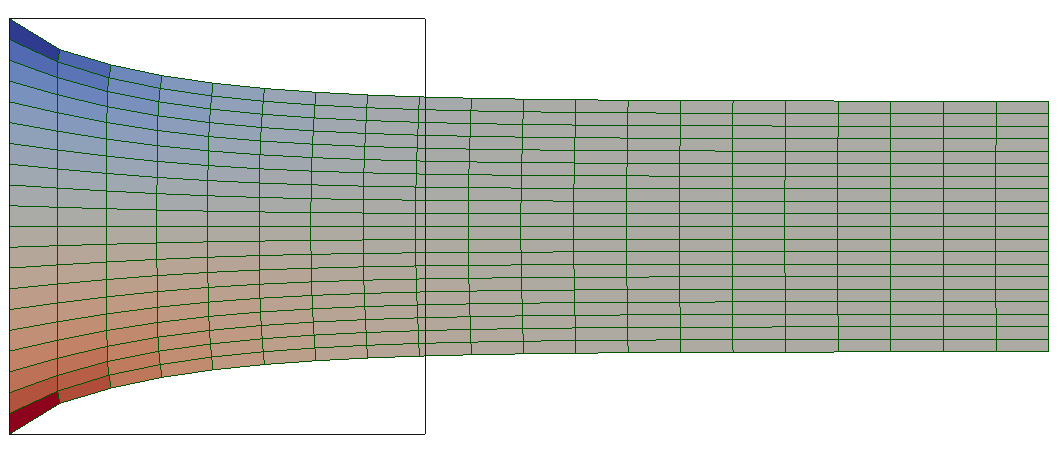
\includegraphics[width=0.7\textwidth]{deformed}
  \caption{Initial geometry and deformed mesh, coloured by the shear
    stress component~$\sigma_{12}$.}
  \label{fig:deformed}
\end{figure}

\subsubsection{Dynamic linear elasticity}
\label{sec:dynamic}

Another special case of the IBVP of elasticity is linear elasticity
which has the assumptions of infinitesimal displacements and a linear
material behaviour. In the dynamic case, this gives the IBVP
\begin{equation}
  \label{eq:dynamic}
  \begin{aligned}
    \rho \partial^2_t \U
    -\nabla \cdot \vek{\sigma} &= \vek{0} \qquad
    &\x &\in \Omega\,, &t &\in [0,T]\\
    \U &= \vek{0}     &\x &\in \Gamma^D\,, &t &\in [0,T]\\
    \vek{\sigma} \cdot \N &= \bar{\vek{g}}
    &\x &\in \Gamma^N\,, &t &\in [0,T]\\
    \U &= \vek{0} &\x &\in \Omega\, &t &< 0
  \end{aligned}
\end{equation}
with the material density~$\rho$, the prescribed (time-dependent!)
traction and the Cauchy stress tensor~$\vek{\sigma}$. Note that under
the simplifications of linear elasticity, there is no need to
distinguish between reference and current configuration nor between the
various stress tensors. The used material simply follows Hooke's law
\begin{equation}
  \label{eq:hooke}
  \vek{\sigma} = \lambda (\nabla \cdot \U) \vek{I} + \mu (\nabla \U +
  \nabla \U^\top)
\end{equation}
and is linear in the gradient of the displacement function~$\U$.  Note
that in problem~\eqref{eq:dynamic} the second time derivative
occurs. Therefore, the quiescent past of the displacement function
for~$t<0$ is used which implies an initial condition of zero
displacement and velocity. Moreover, this second derivative does not
allow a straightforward application of the linear multi-step methods
as given in section~\ref{sec:temporal}. Spatial discretization of the
IBVP~\eqref{eq:dynamic} gives the system of second-order ODEs of the
form
\begin{equation}
  \label{eq:spring}
  \mat{M} \ddot{\mat{x}} + \mat{A} \mat{\x} = \mat{f}\,,
\end{equation}
where the coefficients of the unknown~$\mat{x}$ are still
time-dependent. Now, the velocity $\V = \dot{\U}$ is explicitly
introduced and we obtain the block system
\begin{equation}
  \label{eq:block}
  \begin{pmatrix}
    \mat{0} &\mat{M} \\ \mat{M} &\mat{0} 
  \end{pmatrix}
  \begin{pmatrix}
    \dot{\mat{x}} \\ \dot{\mat{v}} 
  \end{pmatrix} +
  \begin{pmatrix}
    \mat{A} &\mat{0} \\ \mat{0} &-\mat{M} 
  \end{pmatrix}
  \begin{pmatrix}
    \mat{x} \\ \mat{v} 
  \end{pmatrix} =
  \begin{pmatrix}
    \mat{f}  \\ \mat{0} 
  \end{pmatrix} 
\end{equation}
which is a system of first-order ODEs. Now the mechanisms of
section~\ref{sec:temporal} can be applied again.

In this problem, the only non-zero impact on the solid is a horizontal
compressive load on the right side boundary whose non-zero
component~$\bar{g}_1$ has a temporal variation of the type
\begin{equation}
  \label{eq:traction}
  \bar{g}_1(0) = \left\{ 
    \begin{matrix} 
       0 &t < t^* \\
      -1 \cdot 10^4 &t \geq t^* \,,
    \end{matrix}
    \right. 
\end{equation}
that is a step function with jump at some time~$t = t^*$.
Figure~\ref{fig:inp2b} shows the input parameters of the program.
The horizontal displacement~$u_1$ and horizontal velocity~$v_1$
components at the centre point $\x = (0.5,0.5)$ are plotted over time
in figure~\ref{fig:dynamic}. Note that the velocity is scaled in order
to have comparable amplitudes of the curves.

\begin{figure}[htbp]
  \centering
  \begin{minted}[frame=lines]{text}
meshFile       quad.020.smf

# material parameter
E              100000.
nu             0.3

# for dynamic runs
density        1000.
numSteps       500
stepSize       0.002
  \end{minted}
  \caption{Input data of the program.}
  \label{fig:inp2b}
\end{figure}

\begin{figure}[htbp]
  \centering
  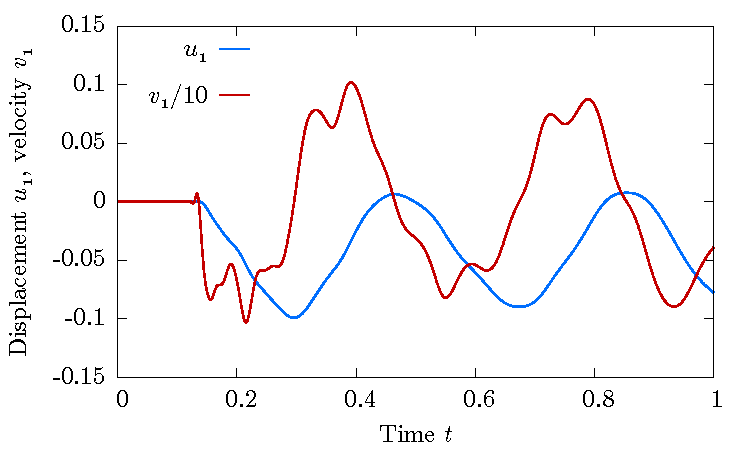
\includegraphics[width=0.7\textwidth]{dynamic}
  \caption{Plot of horizontal displacement and velocity at the centre
    of the domain.}
  \label{fig:dynamic}
\end{figure}

%%------------------------------------------------------------------------------
\newpage
\subsection{Coupled fluid-diffusion}
\label{sec:fluid}

One of the main application goals of \IS{} is multiphysics in which
multiple physical problems interact. As an example, consider a tank
filled with some fluid and within that fluid a certain substance is
transported. We assume that the fluid mechanics of the problem are not
affected by that substance and formulate the fluid IBVP via the
Navier-Stokes equations
\begin{equation}
  \label{eq:navierstokes}
  \begin{aligned}
    \nabla \cdot \V = 0\,, \quad \rho (\partial_t \V + \nabla \V
    \cdot \V) - \mu \nabla^2 \V + \nabla p &= \vek{0} \qquad
    &\x &\in \Omega\,, &t &\in [0,T]\\
    \V &= \bar{\V} &\x &\in \Gamma\,, &t &\in [0,T]\\
    \V &= \bar{0}  &\x &\in \Omega\,, &t &= 0\,.
  \end{aligned}
\end{equation}
The fluid dynamics are described by the velocity field~$\V$ and
pressure~$p$ and, in this case, only velocity boundary conditions are
given on the entire boundary of the domain. Note that the momentum
balance of the Navier-Stokes equations is nonlinear due to the
advection term $\nabla \V \cdot \V$ which will be tackled by a simple
fix point iteration and is not discussed any further. The material
parameters are the mass density~$\rho$ and the fluid viscosity~$\mu$
(assumption of a Newtonian fluid). With the same fluid velocity~$\V$
the transport of the substance's concentration~$c$ is governed by the
IBVP
\begin{equation}
  \label{eq:substance}
  \begin{aligned}
    \rho_s \partial_t c + \V \cdot \nabla c -
    \kappa  \nabla^2 c &= \vek{0} \qquad
    &\x &\in \Omega\,, &t &\in [0,T]\\
    c &= \bar{c} &\x &\in \Gamma\,, &t &\in [0,T]\\
    c &= 0  &\x &\in \Omega\,, &t &= 0
  \end{aligned}
\end{equation}
with the substance's apparent density~$\rho_s$ and the diffusion
constant~$\kappa$. Obviously, problem~\eqref{eq:navierstokes} does not
depend on~$c$ and therefore it can be solved independently. Once the
velocity field~$\V$ is determined, the linear
problem~\eqref{eq:substance} is solved for the latest values of~$c$.

Figure~\ref{fig:inp3} shows the parameter input to the program and
figure~\ref{fig:food} displays the fluid and the diffusion
solutions. The chosen fluid problem is resembles the classic
\emph{driven cavity} numerical benchmark example and one can clearly
see the circulation pattern in the solution. The Reynolds number is
500 for the chosen parameters. On the other hand, the concentration of
the substance is set to zero at all but the top boundaries where a
value of $\bar{c} > 0$ is prescribed. The contour lines in
figure~\ref{fig:food} clearly display how the advection with the fluid
velocity influences the concentration field.

\begin{figure}[htbp]
  \centering
  \begin{minted}[frame=lines]{text}
meshFile   cavity.smf
viscosity  0.002
density    1.00

# non-linear fluid iterations
maxIter    100
tolerance  1.e-5

# time stepping
numSteps   500
stepSize   0.1

# food
kappa        0.002
foodDensity  0.3
foodBoundary 0.5

  \end{minted}
  \caption{Input data of the program.}
  \label{fig:inp3}
\end{figure}

\begin{figure}[htbp]
  \centering
  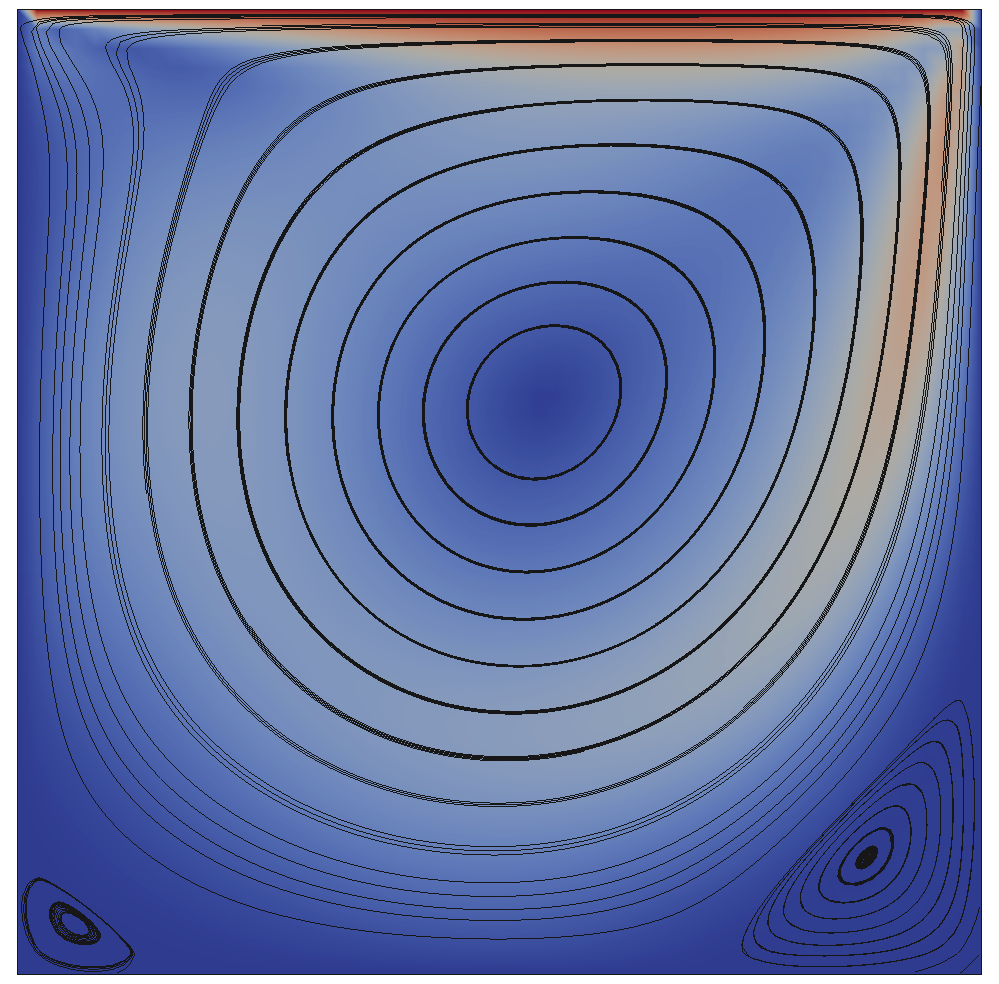
\includegraphics[width=.45\textwidth]{streamlines}\quad
  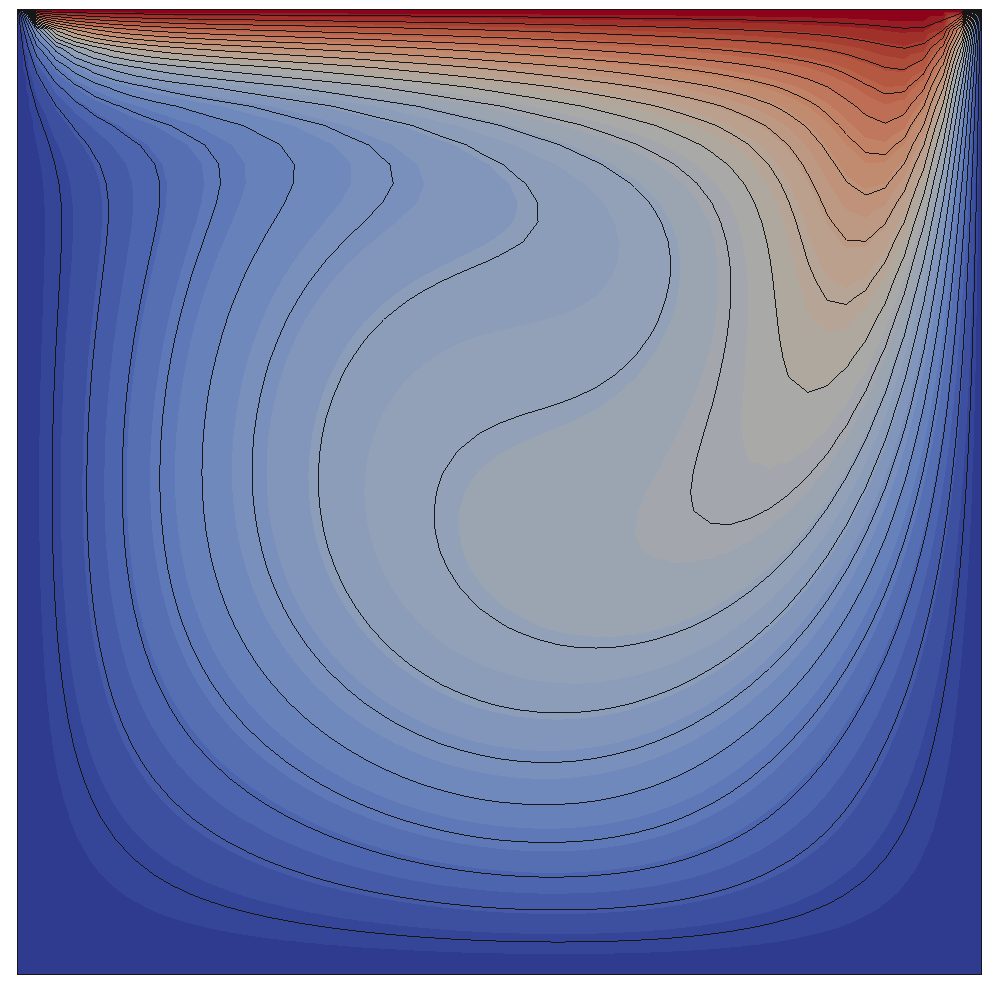
\includegraphics[width=.45\textwidth]{food}
  \caption{Fluid solution with some streamlines (left) and diffusion
    solution with concentration contour lines (right).}
  \label{fig:food}
\end{figure}

\end{document}


%%% Local Variables: 
%%% mode: latex
%%% TeX-master: t
%%% TeX-source-correlate-mode: t
%%% TeX-synctex-tex-flags: "-synctex=1 -shell-escape"
%%% End: 
